\documentclass{article}
\usepackage{tikz, comment}
\usepackage{pifont}
\usepackage{fontspec}
\usetikzlibrary{arrows, decorations.markings, decorations.pathreplacing}
\begin{comment}
:Title: Not defined yet
:Tags: intersection;figure;curves;curve;circle
:Author: Prof.Hu Ji-shan, HKUST
:Slug: No name yet

Description Here.........
\end{comment}
\begin{document}\centering

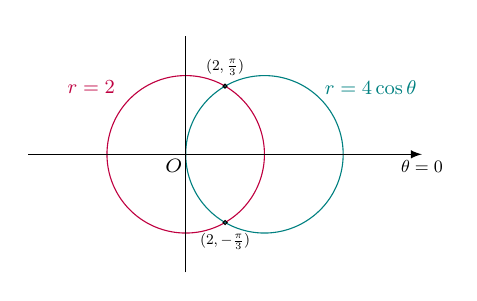
\begin{tikzpicture}[>=latex,xscale=.5*1, yscale=.5*1][font=\sf\small]

%\draw[xstep=1cm,ystep=1cm,color=gray!80] (0, -1) grid (8, 8);

\draw[purple, samples=100, smooth, domain= 0:2*pi, variable=\t]
plot ({2*cos(\t r)}, {2*sin(\t r)});

\draw[teal, samples=100, smooth, domain=0:1*pi, variable=\t]
plot ({4*cos(\t r)*cos(\t r)}, {4*cos(\t r)*sin(\t r)});

\draw[] ({2*cos((pi/3) r)}, {2*sin((pi/3) r)}) circle(0.05)node[above, yshift= 2, scale=0.6]{$(2, \frac{\pi}{3})$};
\draw[] ({2*cos((-pi/3) r)}, {2*sin((-pi/3) r)}) circle(0.05)node[below, yshift=-2, scale=0.6]{$(2, -\frac{\pi}{3})$};

\node[purple, scale=0.8] at (-2.4, 1.7) {$r = 2$};
\node[teal, scale=0.8] at (4.7, 1.7) {$r = 4 \cos \theta$};

\foreach \x in {}
\draw (\x,2pt/6) -- (\x,-2pt/6)
node[anchor=north] {\tiny$\x$}
;

\foreach \x in {}
\draw (\x,2pt/2.5) -- (\x,-2pt/2.5)
node[anchor=south] {\tiny$\x$}
;
\foreach \y in {}
\draw (-2pt/6,\y) -- (2pt/6,\y)
node[anchor=east] {\tiny $\y$}
;

\draw[->] (-4, 0) -- (6, 0)node[below, scale=0.7] {$\theta=0$} ;
\draw[] (0, -3) -- (0, 3)node[left] {};

\node[yshift=0] at (-0.2*1.5, -0.2*1.5) {\scriptsize$O$};

\end{tikzpicture}
\end{document}